
\begin{figure*}[ht!]
	\begin{center}
		%    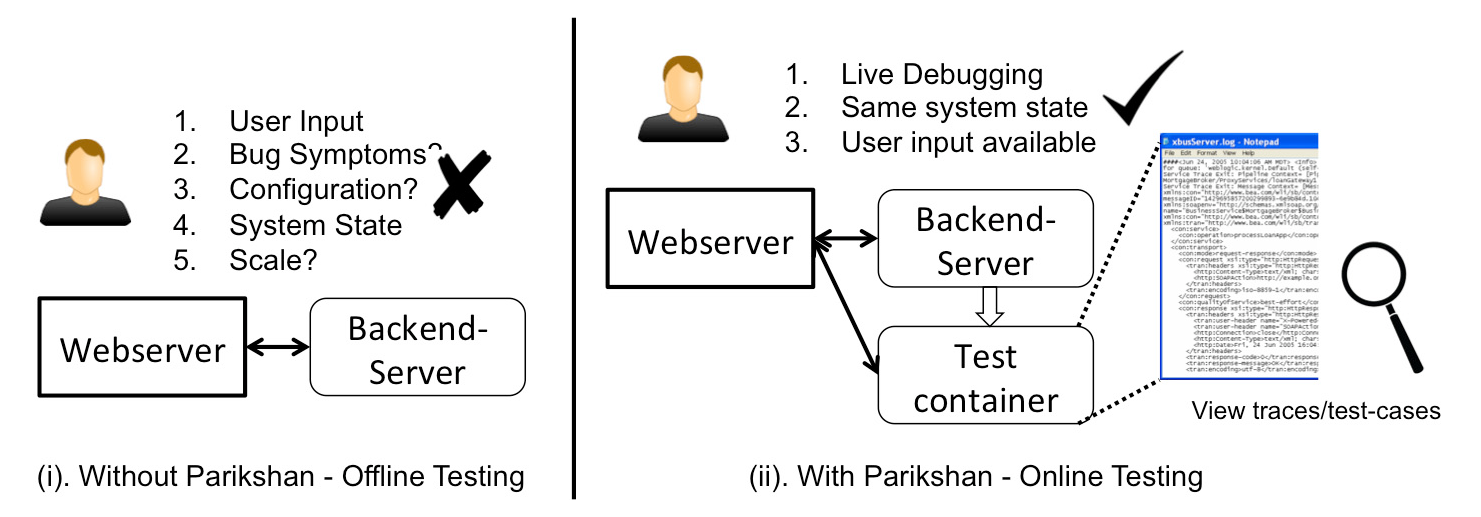
\includegraphics[width=0.7\textwidth]{figs/motivation.eps}
		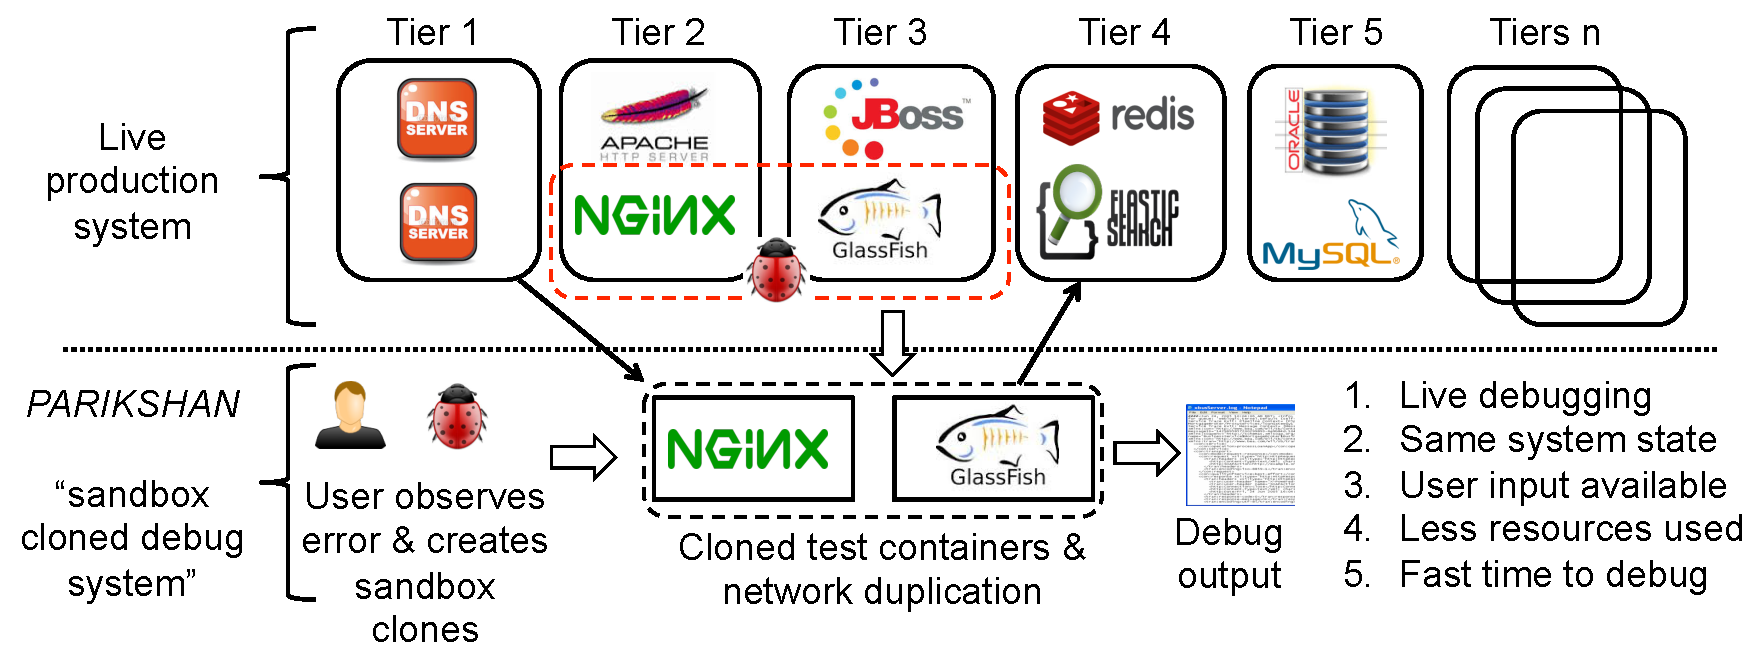
\includegraphics[width=0.9\textwidth]{figs/workflow3.pdf}
		\caption{Workflow of \parikshan in a live multi-tier production system with several interacting services. When the administrator of the system observes errors in two of it's tiers, he can create a sandboxed clone of these tiers and observe/debug them in a sandbox environment without impacting the actual production system.}
		\label{fig:motivation}
	\end{center}
\end{figure*}


\section{Background}
\label{sec:background}

In this section, we give a short description of the design of live debugging and our \parikshan framework to facilitate the exposition of the ideas in this paper. 
%A detailed explanation of the complete design of the paper can be found in ~\cite{parikshan}.

\subsection{The case for Live Debugging}
\label{sec:case}

Figure \ref{fig:motivation}, shows a high level overview of ``live debugging'' in action. 
The figure shows a live production system with multiple services. 
The system is maintained by an operator, who can observe the health of the system using light-weight monitoring, which is part of the deployed system. 
In the interest of application performance, production system monitoring is usually limited to system resource usage, application usage statistics, transaction logs, and error logs.

Let us assume that at a certain time in the execution of the system, the operator observes unusual memory usage in the glassfish application server, and some error logs being generated in the nginx webserver. 
Typically, trouble tickets are generated for such problems, and they are debugged offline.
However, the operator can now use \parikshan to fork off clones of the nginx and glassfish containers as \textbf{nginx-debug} and \textbf{glassfish-debug}.
Network duplication mechanisms ensure that the debug-containers receive the same inputs as the production, and the production containers continue to provide service without interruption.
This seperation of production and debug environments allows the operator to use dynamic instrumentation tools to do deeper diagnosis without fearing any problems in the user-facing operations.
Since the system has been cloned from the original potentially ``buggy'' production container, it will also exhibit the same memory leaks/or logical errors.
Additionally, \parikshan can focus on the ``buggy'' parts of the system, without needing to replicate the entire system in a test-cluster. 
This process will greatly reduce the time to bug resolution, and allow real-time bug diagnosis capability.

\subsubsection{Design Overiview}
\label{sec:designBackground}

Our system called \parikshan, is composed of three modules: 

%\begin{itemize}
%	\item 

 \textbf{Clone Manager}: manages ``live cloning'' between the production and debug containers.
``Live Cloning'' refers to the process of copying a running virtual machine, or container from one server to another, without disconnecting any client or process running within the service.
This generates two containers, a production container which serves the actual user requests, and a debug-container which gets the same input as the production but is maintained only for debugging purposes.
The ``live'' part in the cloning process means that cloning has a very small suspend time and the service is kept active while cloning. \\

\iffalse	
	\begin{figure}[ht]
		\begin{centering}
			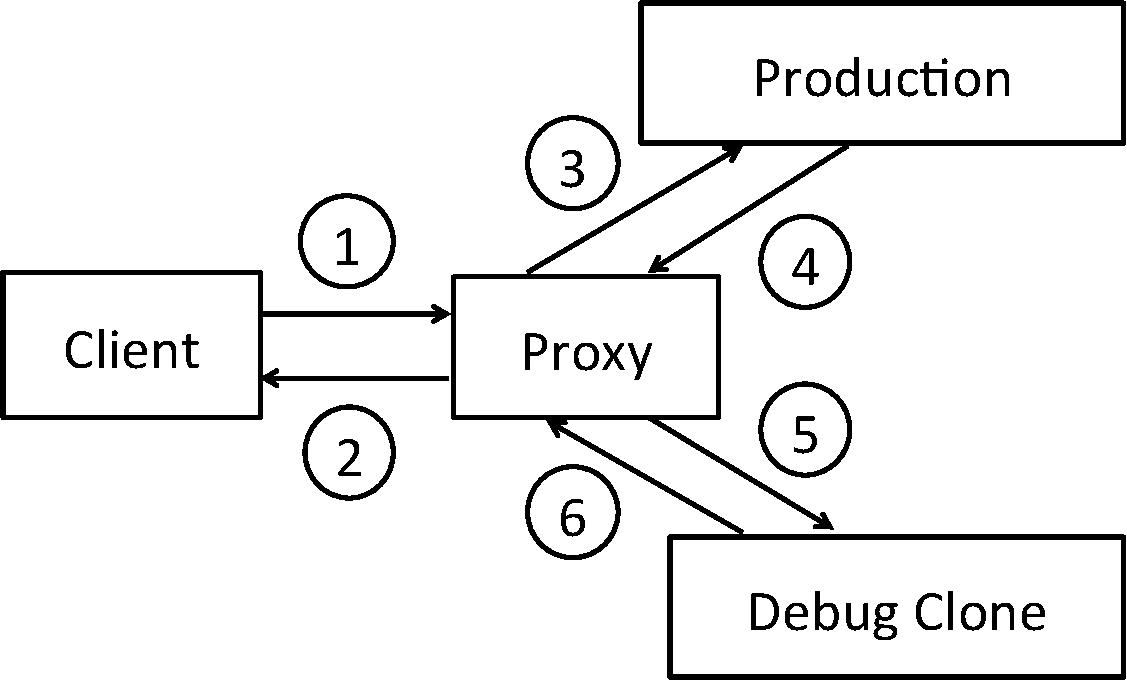
\includegraphics[width=0.4\textwidth]{figs/network_dup.pdf}
			%    \captionsetup{justification=centering}
			\caption{Description of the Network Duplicator. In \textit{synchronized} mode: Thread 1 executes steps [1,3,5], and Thread 2 executes [2,4,6] sequentially. In \textit{asynchronous} mode: Thread 1 executes steps [1,3], Thread 2 executes [2,4], Thread 3 executes [5], and Thread 4 executes [6]}
			\label{fig:duplicator}
		\end{centering}
	\end{figure}
\fi
%\item 
 \textbf{Network Duplicator}: The network duplicator manages communication from the client to both the production container and the debug container.
The basic design is based on a customized TCP level proxy, which duplicates network traffic to both these containers.
As shown in figure~\ref{fig:duplicator}, the duplicator uses an asynchronous packet forwarding model, with 4 threads for each incoming connections.
Thread T1 forwards packets from client to proxy (link 1), and from proxy to production container(link 2). It then uses a non-blocking send to foward packets to an internal pipe buffer shared between thread T1, thread T3. Thread T3, then reads from this piped buffer and sends traffic forward to the debug-container. 
Similarly Thread T2, receives packets from production container, and forwards them to the client, while thread T4, receives packets from debug container and drop them. 

The advantage of this strategy is that any slowdown in the debug-container will not impact the production container.
However, a side-effect is that if the speed of the debug-container is too slow compared to the production container, it may lead to a buffer overflow. 
We call the time taken by a connection before it overflows, it's \textbf{debugging window}.
We assume that both the production and debug containers are identical for the purposes of debugging as long as we do not have an overflow. \\

\textbf{Network Aggregator}: The network aggregator manages communication from 
	
%\end{itemize}
